\documentclass{beamer}

% Theme choice:
\usetheme{Berlin}
\usepackage{tikz-feynman}
\usepackage{array}
\usepackage{animate}
\usepackage{amsmath}
\usepackage{cancel}
\usepackage{multicol}
\usepackage{physics}
\usepackage{graphicx}
\usepackage{amssymb}
\usepackage{hyperref}
%\hypersetup{colorlinks = true,linkcolor = black,filecolor= black,urlcolor= black}
\usepackage{cancel}
\usepackage{subcaption}
\usepackage[super,sort&compress]{natbib}
\usepackage{svg}
\usepackage[toc,page]{appendix}
\author{Vo Chau Duc Phuong}
% Title page details: 
\title{Calculation of the Linear-Absorption Spectrum of\\ an Ideal Two-Dimensional System of $\mathrm{MoS}_2$}
\author{Vo Chau Duc Phuong}
\date{\today}
\logo{\large \LaTeX{}}


\begin{document}
	\small
	% Title page frame
	\begin{frame}
		\titlepage 
	\end{frame}
	
	% Remove logo from the next slides
	\logo{}
	
	
	% Outline frame
	\begin{frame}{Outline}
		\tableofcontents
	\end{frame}
	
	
	% Lists frame
	\section{Overview}	
	
	
	\begin{frame}{Transition Metal Dichalcogenides Monolayer}
		Group VI-B Transition Metal Dichalcogenides (TMD) are compound semiconductors of the type $MX_2$. $M$ is Transition Metal atom (black dots), $X$ are Dichalcogenides atom (green dots):
		\begin{figure}
			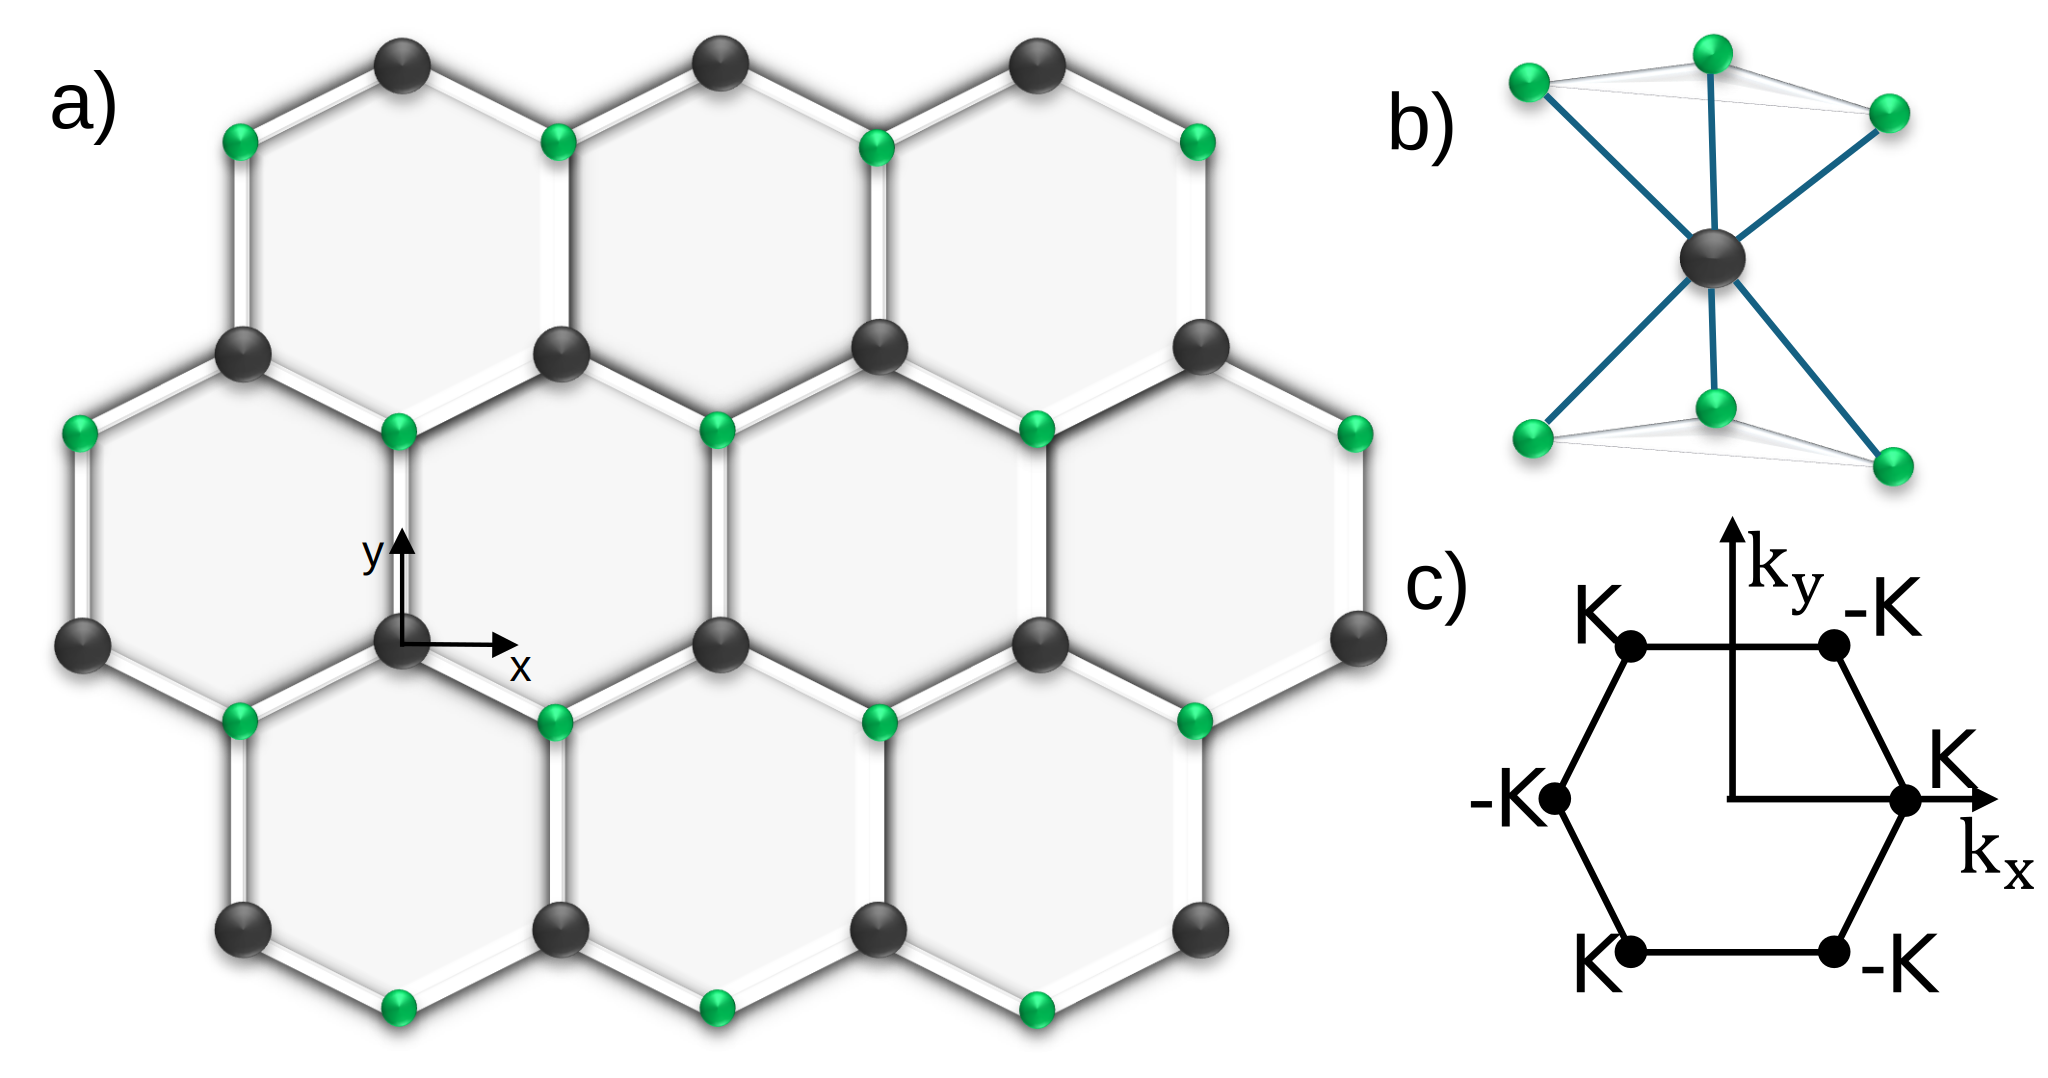
\includegraphics[width=0.4\linewidth]{images/RS.pdf}
		\end{figure}
		\begin{itemize}
			\item They stable in both mono- and few-layer in the air at room temperature.\\
			\item They are semiconductor with a direct band gap.\\
			\item Strong spin-orbit Coupling (SOC) in TMD monolayers leads to spin splitting of hundreds meV.
		\end{itemize}
	\end{frame}
	\begin{frame}{Exciton Binding Energy In TMD}
		Why calculate the linear absorption spectrum?\\ $\to$ Exciton Binding Energy
		\begin{itemize}
			\item TMD is a low-dimension material, create huge binding energy in compare with bulk semiconductor $\to$ huge effect on phenomenon $\Rightarrow$ need to be calculated and taken into account in any further many-body calculation.
			\item Early theories predict binding energy too large ($0.5-1$ eV) in compare with experiment ($0.2-0.5$ eV) $\Rightarrow$ need precise calculation in agree with experiment.
			\item Other theory only fitting bandstructure around high symmetry point such as $K/K'$, not on entire BZ $\Rightarrow$ Tight-Binding method for fitting on entire BZ.
		\end{itemize}
	\end{frame}
	% Blocks frame
	\section{Method}
	\subsection{Three-band Tight-binding Model}
	\begin{frame}
		Tight-Binding (TB) wave function have the form of Linear combination of Atomic Orbital (LCAO):
		\begin{equation}
			\ket{\psi_{\lambda \textbf{k}}(\textbf{r})} = \sum_{\alpha} c_{\lambda \alpha} (\textbf{k}) \sum_{\textbf{R}} e^{i\textbf{k}\textbf{R}} \ket{\phi_{\alpha}(\textbf{r}-\textbf{R})}
		\end{equation}
		Time-independence independence-electron approximation Schrödinger equation with LCAO included:
		\begin{equation*}
			H_{1e} \sum_{\alpha} c_{\lambda \alpha} (\textbf{k}) \sum_{\textbf{R}} e^{i\textbf{k}\textbf{R}} \ket{\phi_{\alpha}(\textbf{r}-\textbf{R})} = \varepsilon_{\lambda} (\textbf{k}) \sum_{\alpha} c_{\lambda \alpha} (\textbf{k}) \sum_{\textbf{R}} e^{i\textbf{k}\textbf{R}} \ket{\phi_{\alpha}(\textbf{r}-\textbf{R})}
		\end{equation*}
		Multiply with $\bra{\phi_{\beta}}$ on the left and take integral over $\textbf{r}$
		\begin{equation}
			\sum_{\alpha} [H^{TB}_{\beta \alpha}(\textbf{k}) - \varepsilon_{\lambda}(\textbf{k})\delta_{\beta\alpha}]c_{\lambda \alpha}(\textbf{k}) = 0.
		\end{equation}
		In which the Tight-binding Hamiltonian matrix elements:
		\begin{equation}
			H^{TB}_{\beta \alpha}(\textbf{k}) = \sum_{\textbf{R}} \bra{\phi_{\beta} (\textbf{r})} H_{1e}\ket{\phi_{\alpha}(\textbf{r}-\textbf{R})}
		\end{equation}
	\end{frame}
	\begin{frame}
Use basic functions of d-type Orbitals: $$\ket{\phi_1} = d_{z^2}, \ket{\phi_2} = d_{xy}, \ket{\phi_3} = d_{x^2- y^2}.$$\\Three-band TB Hamiltonian with SOC has the form:
		\begin{equation}
			H^{TB}_{6\times 6}(\textbf{k}) = \begin{bmatrix}
				H^{TB}_{3\times 3}(\textbf{k}) + \gamma L_z & 0\\ 0& H^{TB}_{3\times 3}(\textbf{k}) - \gamma L_z
			\end{bmatrix}, \quad L_z= \begin{bmatrix}
			0 & 0 & 0\\
			0 & 0 & i\\
			0 & -i& 0
			\end{bmatrix}
		\end{equation}
		\begin{figure}			
			\includegraphics[width=0.5\linewidth]{images/BS.pdf}
			\caption{$MoS_2$ Bandstructure calculated from 3-band TB models\cite{liu_three-band_2013}}
		\end{figure}
	\end{frame}
	\subsection{Semiconductor Bloch Equations}
	\begin{frame}
	Multiband velocity gauge semiconductor Bloch equations (SBE) with Coulomb interaction in Hatree Fock approximation:
	\begin{align}
		\dv{ }{t}\rho_{\lambda \lambda'} (\textbf{k},t) = &-\frac{i}{\hbar} (\varepsilon_{\lambda}(\textbf{k}) -\varepsilon_{\lambda'}(\textbf{k}))\rho_{\lambda \lambda'} (\textbf{k})\nonumber\\
		& -i \sum_{\mu} (\Omega_{\lambda \mu}(\textbf{k})\rho_{\mu \lambda'}(\textbf{k},t) -\rho_{\lambda \mu}(\textbf{k},t)\Omega_{\mu \lambda'}(\textbf{k}))\\
		& + \frac{\rho_{\lambda \lambda'}(\textbf{k},t)}{T_2}(1-\delta_{\lambda\lambda'}),\nonumber
	\end{align}
	where
	\begin{align}
		\Omega_{\mu \nu}(\textbf{k}) = &\frac{1}{\hbar} \bigg(\frac{e}{m}\textbf{A}(t)\textbf{p}_{\mu \nu}(\textbf{k}) - \sum_{\alpha \beta \textbf{q}} W^{\alpha \mu \beta\nu}_{\textbf{k},\textbf{k}+\textbf{q},\textbf{q}}\rho_{\beta\alpha}(\textbf{k}+\textbf{q})\bigg),\\
		&\textbf{p}_{\mu\nu}(\textbf{k}) = \frac{m}{\hbar}\sum_{\alpha,\beta} c^*_{\mu\alpha}\nabla_{\textbf{k}}H^{TB}_{\alpha\beta}(\textbf{k})c_{\nu\beta}(\textbf{k})
	\end{align}
	\end{frame}
\subsection{Inter-band Polarization}
\begin{frame}
		\begin{multicols}{2}
For $\mu \neq \nu$:
			\begin{equation}
\vec{\xi}_{\mu\nu}(\textbf{k}) = \frac{-i\hbar}{m}\frac{\textbf{p}_{\mu\nu}(\textbf{k})}{\varepsilon_{\mu}(\textbf{k}) - \varepsilon_{\nu}(\textbf{k})}
			\end{equation}
Time-dependence interband polarization density:
	\begin{align}
		\textbf{P}(t) = &\frac{e}{L^2} \sum_{\textbf{k}} \Tr\bigg[\vec{\xi}(\textbf{k})\rho(\textbf{k},t)\bigg]\nonumber\\
		= &\frac{e}{L^2} \sum_{\textbf{k}\lambda\lambda'}\vec{\xi}_{\lambda\lambda'}(\textbf{k})\rho_{\lambda'\lambda}(\textbf{k},t)
	\end{align}
			\columnbreak
			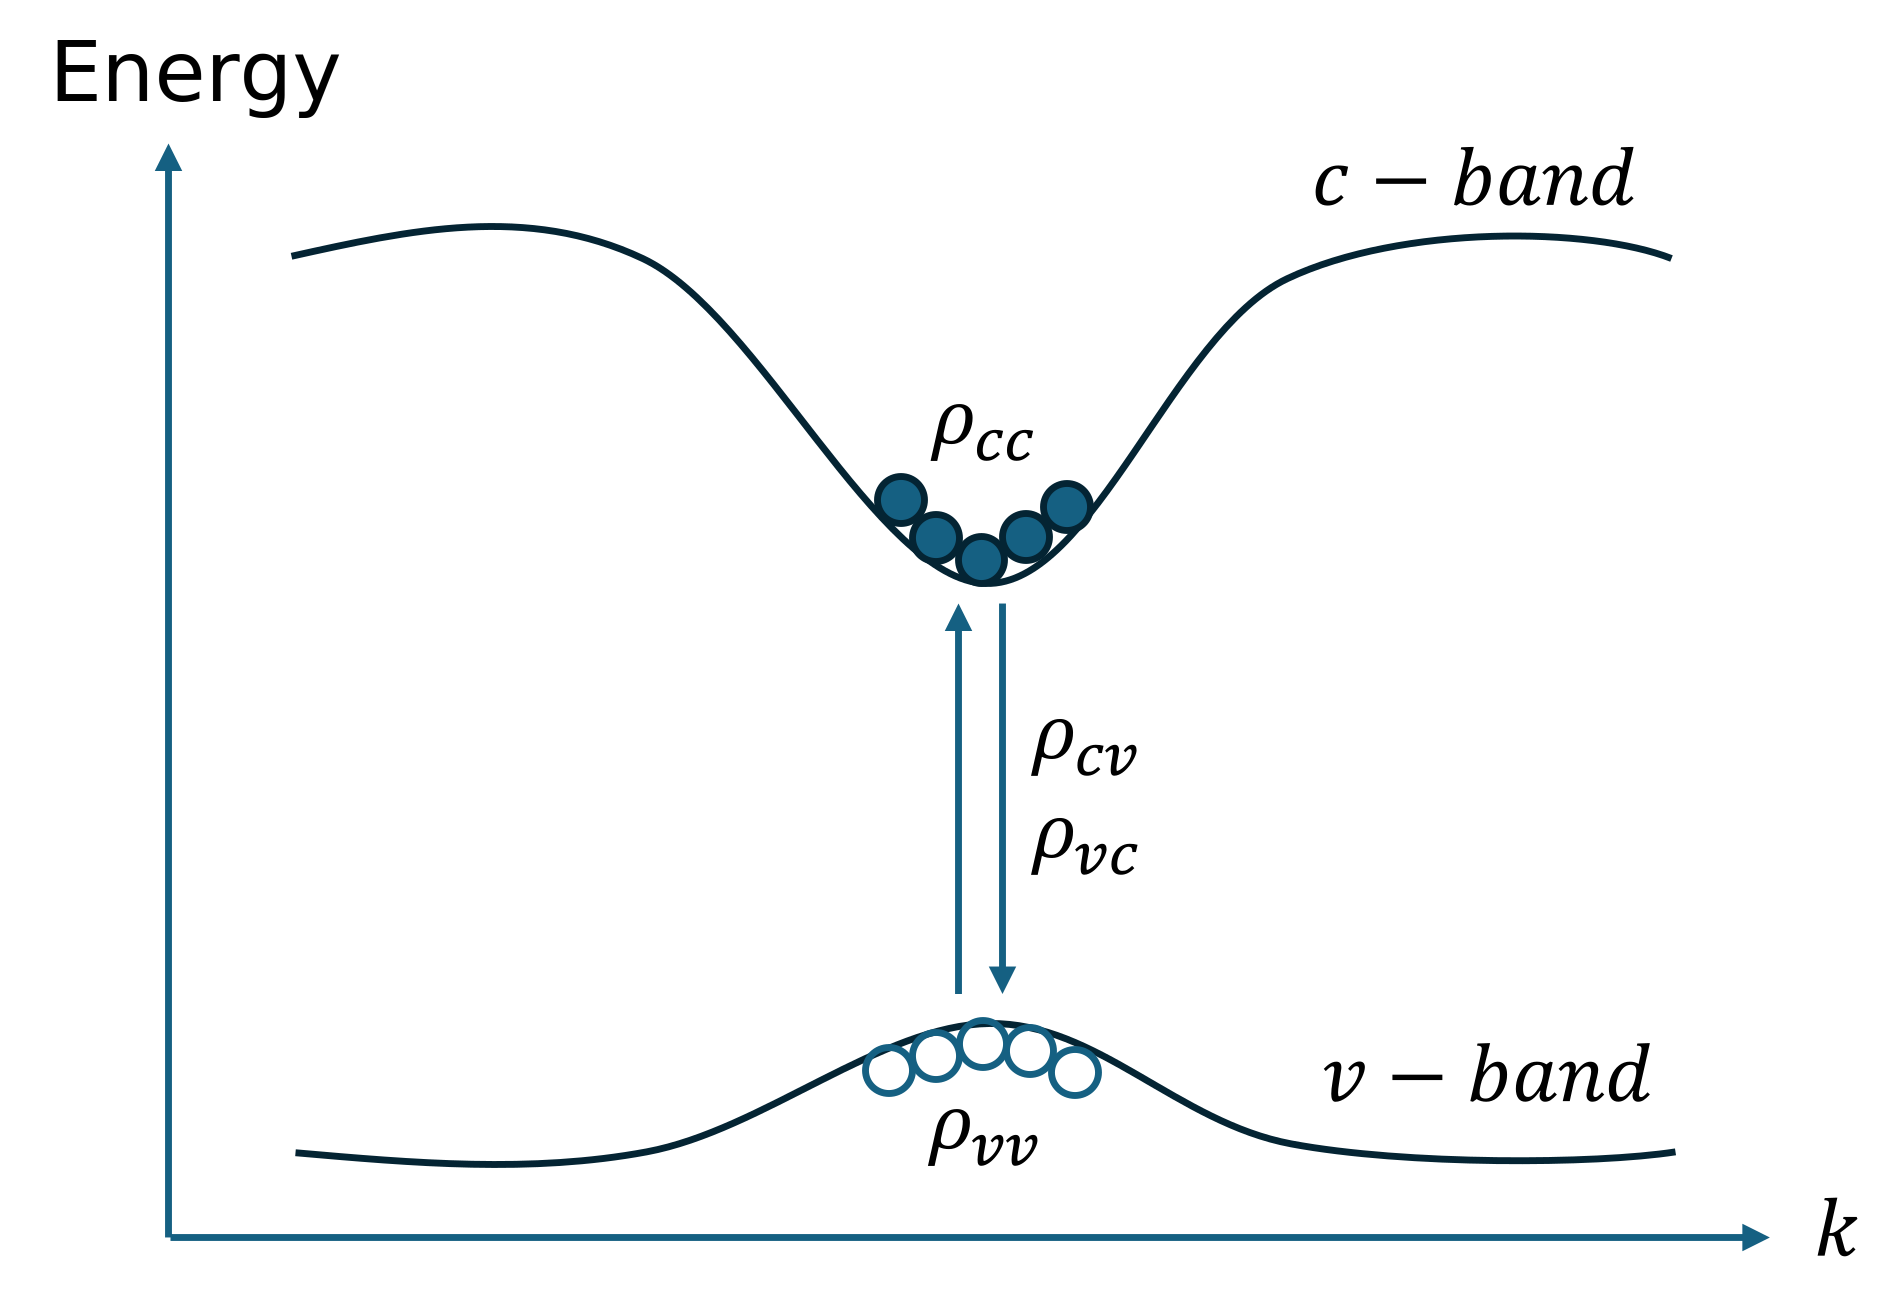
\includegraphics[width=0.8\linewidth]{images/cvbeamer.pdf}
		\end{multicols}
	\end{frame}
\section{Numerical Results}
	\begin{frame}{Numerical Sum Over k-Space}
		\begin{figure}
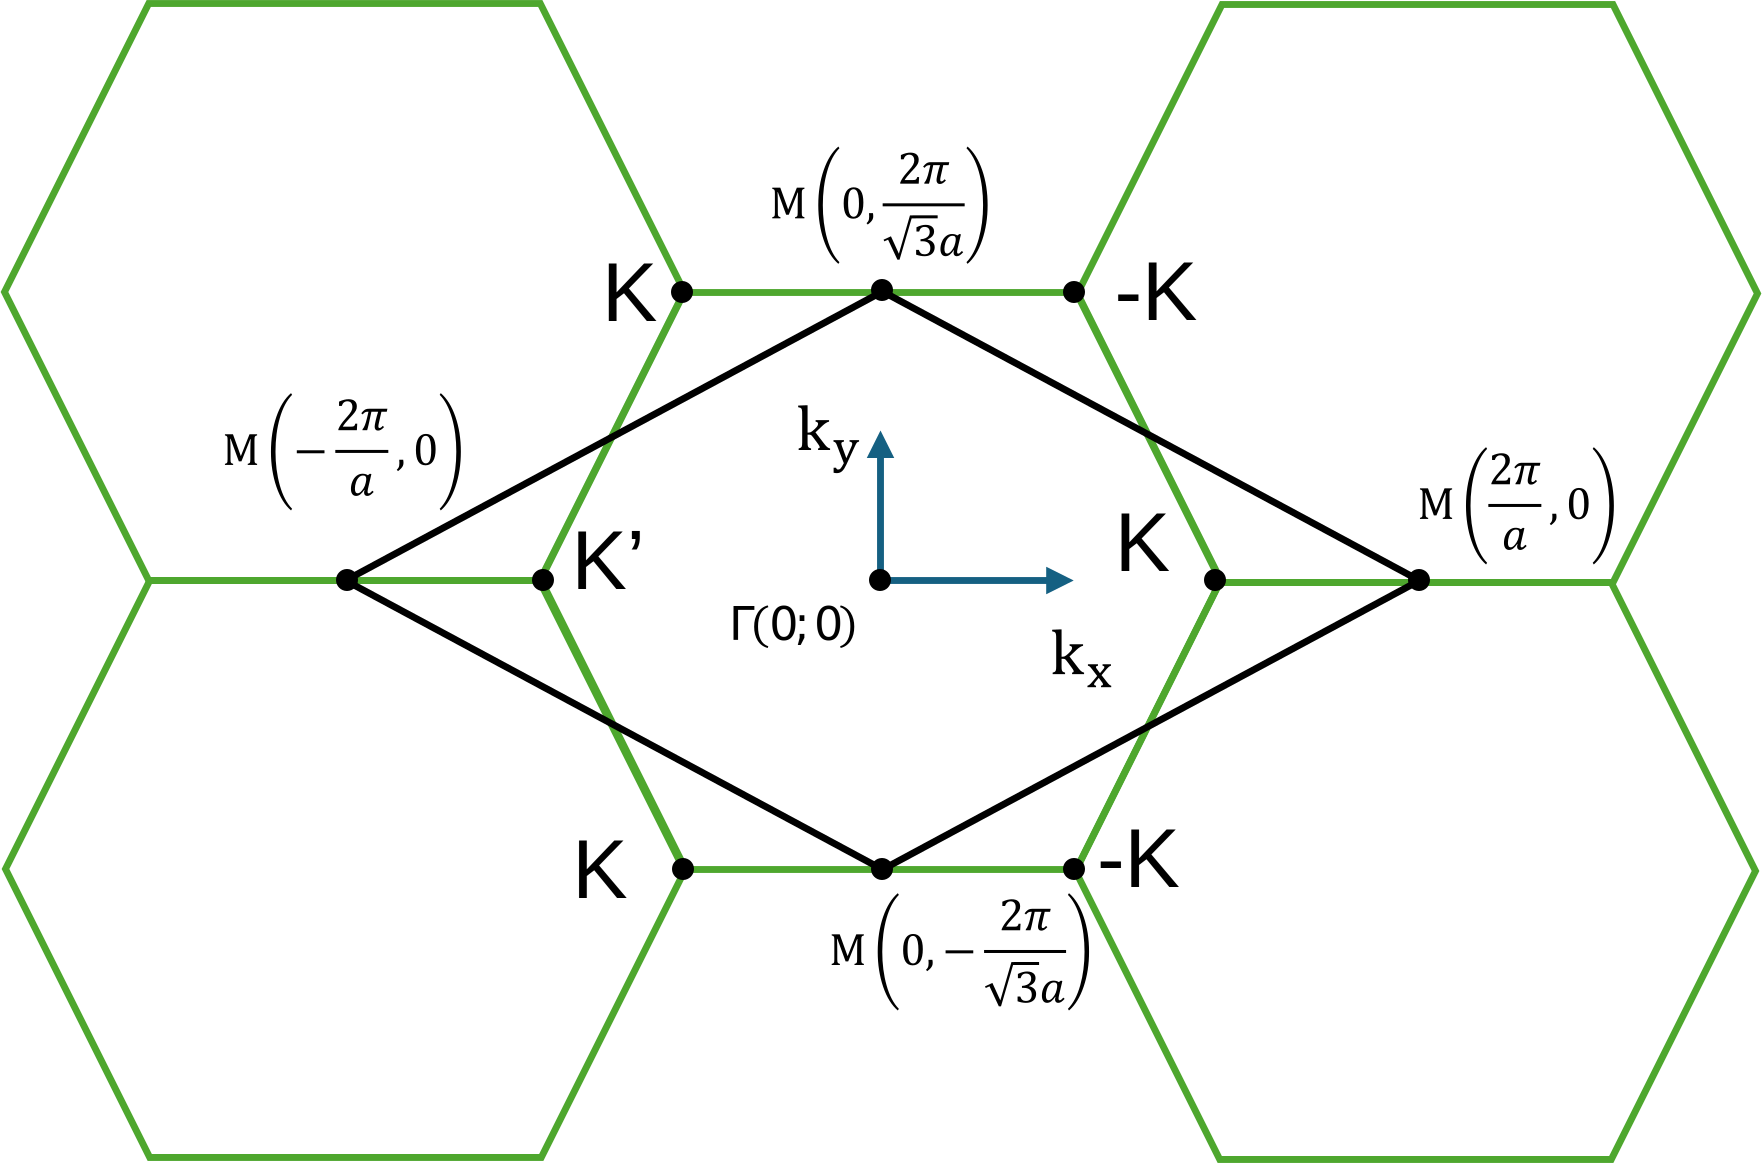
\includegraphics[width=0.5\linewidth]{images/Rhombus.pdf}
\end{figure}
		\begin{equation}
			\sum_{\textbf{k}} ... \to \frac{L^2}{4\pi^2} \int \int_{BZ} dk_x dk_y...
		\end{equation}
	\end{frame}
	\begin{frame}{k-Cutoff}
	\begin{figure}		
		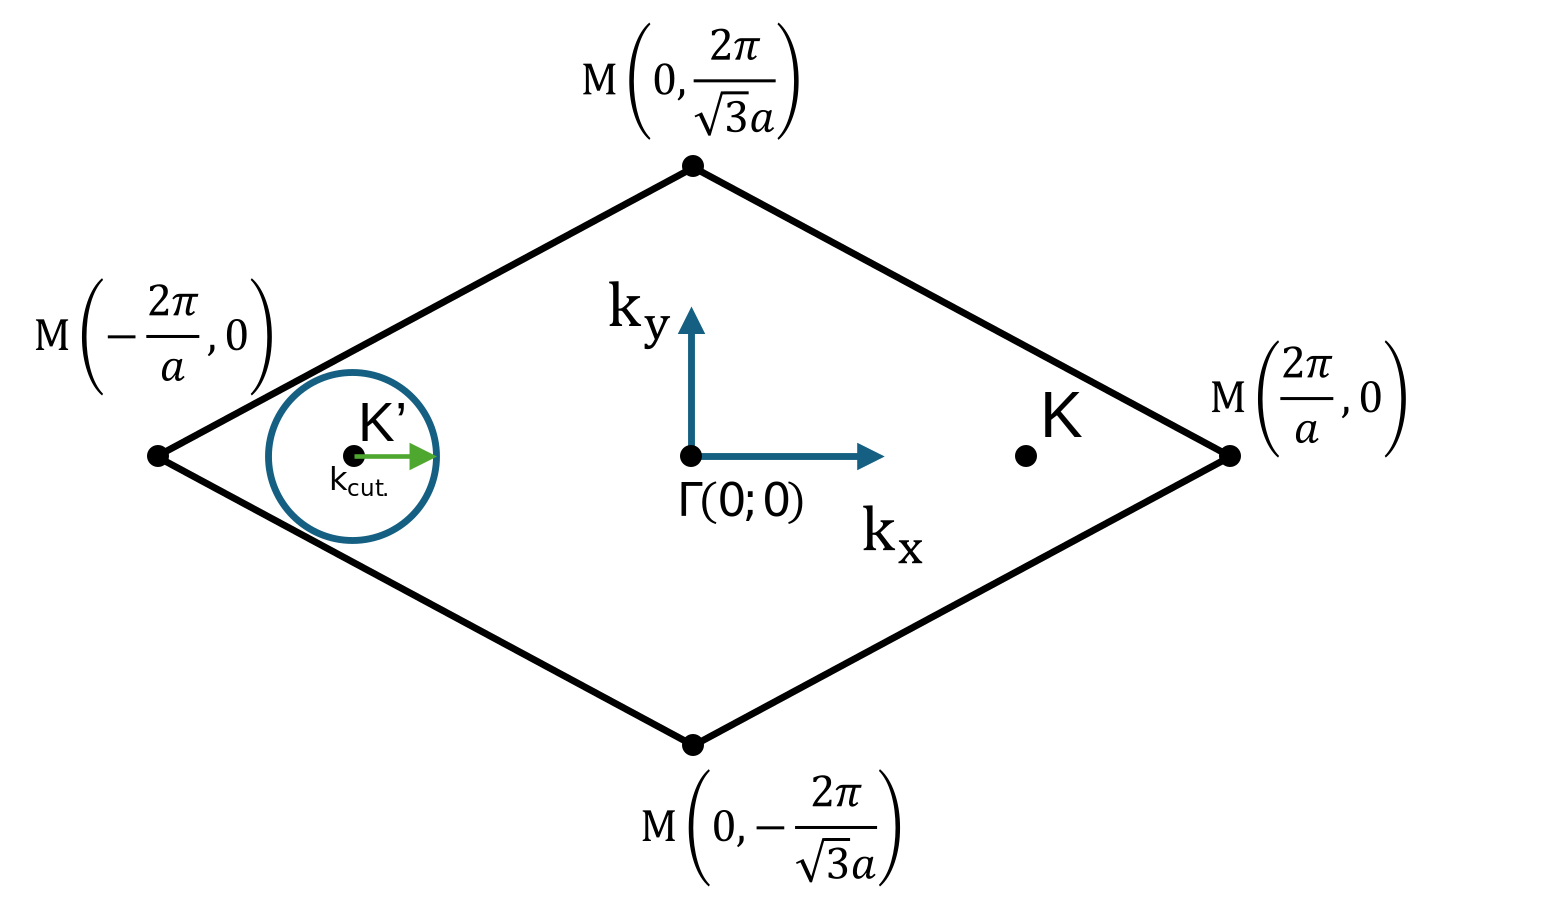
\includegraphics[width=0.75\linewidth]{images/kcutoff.pdf}
	\end{figure}
	\begin{equation}
		W^{\alpha \mu \beta \nu}_{\textbf{k},\textbf{k}',\textbf{q}} \approx W^{\alpha \mu \beta \nu}_{\textbf{k},\textbf{k}',\textbf{q}} \theta(k_{cut.} - |\textbf{k} - \textbf{k}_{K'}|) \theta(k_{cut.} - |\textbf{k}' - \textbf{k}_{K'}|).
	\end{equation}
	\end{frame}
	\begin{frame}{Electromagnetic Field}
	\begin{multicols}{2}
Electromagnetic has Gaussian form:
\begin{equation}
	\textbf{E}(t) = \textbf{E}_0 \cos(\omega t)e^{-\frac{t^2}{\tau_L^2}}
\end{equation}
\begin{itemize}
	\item small $E_0: \rho_{cc}(\textbf{k}) \to 0$
	\item $\hbar \omega = E_{gapp.} \to $ linear absorption
	\item small $\tau_L$ for better range around $\omega$
\end{itemize}
\columnbreak
\includegraphics[width=1\linewidth]{images/Eat.pdf}

Absorption obtain by\cite{haug_quantum_2009}:
\begin{equation}
	\alpha(\omega) \propto \frac{P(\omega)}{E(\omega)}
\end{equation}
	\end{multicols}
	\end{frame}
	\begin{frame}
		Experiment measure:
		\begin{multicols}{2}
		\begin{figure}
	\includegraphics[width = 1\linewidth]{images/Experiment.pdf}
	\caption{Measure Absorption Spectrum of $\mathrm{MoS}_2$ at $T=5K$  extracted from \cite{zhang_absorption_2014}}
	\end{figure}
	\columnbreak
	\begin{itemize}
		\item Two resonance labeled by A and B is Exciton peak. Show band split by SOC
		\item Small trion peak near A label by A'
	\end{itemize}
	\end{multicols}
	\end{frame}
\begin{frame}
	\includegraphics[width=0.8\linewidth]{images/varyepsilon.pdf}
	\begin{itemize}
		\item Choosing the $\varepsilon$ for fitting with experiment.
		\item For 3-band TB model: $\varepsilon \in (1.5,2.5)$ is good with Exciton binding energy $E_{bind.}= 0.2-0.5 eV$ 
	\end{itemize}
\end{frame}
\begin{frame}
		\begin{figure}
			\includegraphics[width=0.8\linewidth]{images/varyT2.pdf}
		\end{figure}
	
	\begin{itemize}
	\item Choosing the $T_2$ for clearer Exciton peak.
	\item The bigger $T_2$, the clearer main Exciton peaks $\to $ confirm.
	\item At $T_2 = 30 fs$ show other smaller exciton peaks $\to $ predict.
	\end{itemize}
\end{frame}
	%\begin{frame}
	%\includegraphics[width=1\linewidth]{images/varynk.pdf}
	%\end{frame}
	\section{Summary and Outlook}
	\begin{frame}
		Summary:
		\begin{itemize}
	\item From three-band TB + SBE $\to $ Linear Absorption Spectrum
	\item Confirm on Exciton binding energy in monolayer $\mathrm{MoS}_2$ in contract with experiment, predict smaller exciton peaks.
		\end{itemize}
	Further research:
	\begin{itemize}
		\item High Harmonic Generation
		\item High-order Side-band Generation
		\item Photovoltaic effect
	\end{itemize}
	\end{frame}
	\begin{frame}
		
		\bibliographystyle{ieeetr}
		\bibliography{library}
	\end{frame}
\end{document}